\PassOptionsToPackage{unicode=true}{hyperref} % options for packages loaded elsewhere
\PassOptionsToPackage{hyphens}{url}
%
\documentclass[]{article}
\usepackage{lmodern}
\usepackage{amssymb,amsmath}
\usepackage{ifxetex,ifluatex}
\usepackage{fixltx2e} % provides \textsubscript
\ifnum 0\ifxetex 1\fi\ifluatex 1\fi=0 % if pdftex
  \usepackage[T1]{fontenc}
  \usepackage[utf8]{inputenc}
  \usepackage{textcomp} % provides euro and other symbols
\else % if luatex or xelatex
  \usepackage{unicode-math}
  \defaultfontfeatures{Ligatures=TeX,Scale=MatchLowercase}
\fi
% use upquote if available, for straight quotes in verbatim environments
\IfFileExists{upquote.sty}{\usepackage{upquote}}{}
% use microtype if available
\IfFileExists{microtype.sty}{%
\usepackage[]{microtype}
\UseMicrotypeSet[protrusion]{basicmath} % disable protrusion for tt fonts
}{}
\IfFileExists{parskip.sty}{%
\usepackage{parskip}
}{% else
\setlength{\parindent}{0pt}
\setlength{\parskip}{6pt plus 2pt minus 1pt}
}
\usepackage{hyperref}
\hypersetup{
            pdftitle={Risk Benefit Analysis for Toast-USB Launch},
            pdfauthor={Allison McCarty, Nicholas Mobley, Nijia Ke},
            pdfborder={0 0 0},
            breaklinks=true}
\urlstyle{same}  % don't use monospace font for urls
\usepackage[margin=1in]{geometry}
\usepackage{graphicx,grffile}
\makeatletter
\def\maxwidth{\ifdim\Gin@nat@width>\linewidth\linewidth\else\Gin@nat@width\fi}
\def\maxheight{\ifdim\Gin@nat@height>\textheight\textheight\else\Gin@nat@height\fi}
\makeatother
% Scale images if necessary, so that they will not overflow the page
% margins by default, and it is still possible to overwrite the defaults
% using explicit options in \includegraphics[width, height, ...]{}
\setkeys{Gin}{width=\maxwidth,height=\maxheight,keepaspectratio}
\setlength{\emergencystretch}{3em}  % prevent overfull lines
\providecommand{\tightlist}{%
  \setlength{\itemsep}{0pt}\setlength{\parskip}{0pt}}
\setcounter{secnumdepth}{0}
% Redefines (sub)paragraphs to behave more like sections
\ifx\paragraph\undefined\else
\let\oldparagraph\paragraph
\renewcommand{\paragraph}[1]{\oldparagraph{#1}\mbox{}}
\fi
\ifx\subparagraph\undefined\else
\let\oldsubparagraph\subparagraph
\renewcommand{\subparagraph}[1]{\oldsubparagraph{#1}\mbox{}}
\fi

% set default figure placement to htbp
\makeatletter
\def\fps@figure{htbp}
\makeatother


\title{Risk Benefit Analysis for Toast-USB Launch}
\author{Allison McCarty, Nicholas Mobley, Nijia Ke}
\date{3/18/2021}

\begin{document}
\maketitle

\hypertarget{abstract}{%
\subsection{Abstract}\label{abstract}}

The popularity of toast as an American breakfast food as well as recent
trends in technology have created a potential marketspace for the
Toast-USB, which allows individuals to curate gourmet toast straight
from their computer. We performed a risk-benefit analysis on two samples
obtained by our firm's Department of Experiments (DOE) to investigate
the potential favorable response rate for the product as well as
potential target demographic groups for the marketing campaign. A series
of logistic models were built to investigate the potential success of
this product. We found that the best logistic model included demographic
variables representing loan, age, default, and education as demographic
indicators of interest. However, the favorable response rate for the
product was 12.14\%, which was roughly half of the necessary response
rate required for launch of the product. Thus, based on this
risk-benefit analysis, we do not recommend that Toast-Co move forward
with this campaign. However, we do have some actionable next-step
suggestions for Toast-Co to implement to continue their exploration in
this exciting market space.

\hypertarget{introduction}{%
\subsection{Introduction}\label{introduction}}

Toast has been a staple in the American breakfast for many decades.
Avocado and hummus toast has also been the center of Millennial and
Gen-Z dietary trends, creating a surge in the popularity of gourmet
toast. The sustained popularity of toast as a breakfast food coupled
with a recent drive in demand for gourmet toast created a potentially
high-potential market space to combine toast with technology. Our
client, Toast Co., is aiming to capitalize on a first-mover advantage
and explore this new potential market space. Thus, Toast Co., has
created the Toast-USB which enables individuals to curate gourmet,
artisanal toast right from their computer.

Our aim is to assist Toast Co.~to make informed, data-driven decisions
regarding the launch of Toast-USB. Toast Co.~conducted a first round
market analysis from five metropolitan areas (including Toronto, ON; New
York City, NY, Philadelphia, PA; Dallas, TX, and San Francisco, CA).
Preliminary results were so promising that our firm's DOE has conducted
another larger-scale study to determine the likelihood of success of
Toast-USB. During the course of this investigation, we will synthesize
the key findings from the first and second study. This includes
significant data processing to both reconcile the data of the first and
second study, as well as to process demographic data such that it can be
used in model analysis. Further exploratory analysis will be performed
to investigate key demographic groups that are significant predictors of
a favorable response rate. To perform a risk-benefit analysis on
continuation of the campaign, we will build a series of logistic models
using demographic predictors of interest, and use cross validation based
on maximizing the likelihood ratio to select the model. The model
selection should provide insight on which demographic groups should be
targeted by the marketing campaign, should Toast Co.~move forward with
the launch. Next, we will predict the favorable response rate based on
the selected model, and give a binary(Y/N) recommendation on launch of
the product. Finally, we will determing an MSRP for the product using a
simulation of the logistic model.

\hypertarget{the-data}{%
\subsection{The Data}\label{the-data}}

The original dataset obtained from Toast Co.'s market analysis contained
421 observations of 8 variables, including 6 categorical variables and 2
numeric variables. The data used for supplementary analysis was provided
by our firm's DOE where additional respondents were sampled from the
same 5 major metropolitan areas to supplement the initial campaign,
which gathered information on 45,211 observations for 16 different
variables, including 9 categorical variables and 7 numeric variables.
Variables relating to the demographic information of the respondents
were all self reported, while variables pertaining to duration of
contact and number of contacts were recorded by campaign administers.
Description of all variables can be found in the data dictionary of the
appendix.

\hypertarget{examining-missing-data}{%
\subsubsection{Examining Missing Data}\label{examining-missing-data}}

From the given data there are 45,211 observations. However there are
17,216 (38.10\%) observations that contain one or more missing values.
Certain categorical variables had missing values with no clear pattern
of missingness. These variables included job, education, contact,
previous days from contact, personal loan status, default status,
marital status, and education. With these variables we decided to add
another category termed ``Unknown'' to represent observations where the
respondents elected to either not respond or were unable to provide
adequate information. However we still needed to address observations
that had missing values in the continuous variables.

We first wanted to understand if the continuous variables were missing
in any distinct pattern. From Figure 1, it appears that the data is
missing at random. In Figure 1, the red cells represent variables that
are missing for a specific pattern, while the numbers on the left
represent how many instances that pattern appeared in the data set. The
number at the bottom of the graphic represents the total number of times
the variable of the column was missing. The graphic suggests that we
only observed 3 rows in which the pattern had 3 missing variables at
once. These three patterns only appeared 13 times in our data set. The
infrequency of these patterns signify that these patterns did occur
randomly. Furthermore, there were 6 distinct patterns that were missing
2 or more variables with a total of 439 occurrences. Since all the
patterns of missing data occurred with a low frequency, it is assumed
that all of our missing values are missing at random. This reinforces
that the quality of sampling and surveying conducted by the DOE, as well
as gives us the freedom to either delete or impute the missing values
without the worry of skewing the data inappropriately.

\begin{figure}
\centering
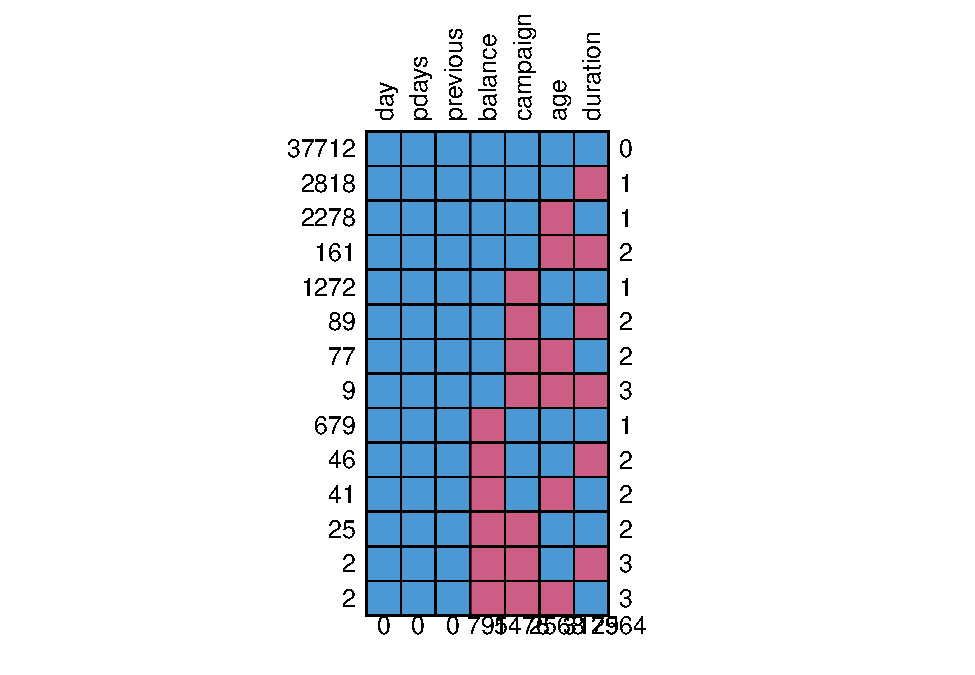
\includegraphics{CompiledTechnicalReport_files/figure-latex/unnamed-chunk-1-1.pdf}
\caption{Missingness pattern of continuous variables in the second
study}
\end{figure}

\hypertarget{imputing-continous-variables}{%
\subsubsection{Imputing Continous
Variables}\label{imputing-continous-variables}}

After determining that the four variables containing missing values
(balance, campaign, age, and duration) were all missing at random, we
decided to address this issue by performing a single imputation of the
median to replace the missing values. We conducted an imputation, as
opposed to deleting all observations with missing data in an attempt to
preserve the information of the other 15 variables in these 7,964
observations.

We determined that the median, as opposed to the mean, was the
appropriate measurement to impute the values since all the variables of
interest except age where all right-skewed. Because the variables were
skewed, replacing the missing values with the mean would have
drastically shifted the imputed data sets distributions farther to the
right than expected. This median is not susceptible to skewness meaning
the new imputed distributions will be representative of the original
data set.

\newpage

\hypertarget{comparison-of-demographic-features-for-the-two-studies}{%
\subsection{Comparison of Demographic Features for the Two
Studies}\label{comparison-of-demographic-features-for-the-two-studies}}

\hypertarget{graphic-comparison-for-the-first-and-second-study}{%
\subsubsection{Graphic Comparison for the First and Second
Study}\label{graphic-comparison-for-the-first-and-second-study}}

We first compare the demographic features common in both studies,
including two numeric variables age and non-mortgage loan balance, as
well as five categorical variables job, education, marital status,
mortgage and primary phone.

To determine whether the decision to purchase the product is
statistically associated with the numeric variable age in the second
study, we generated a boxplot to compare the age distribution of
respondents who are willing to purchase the product against those who
are not. As is shown in Figure 2, people who are willing to purchase the
product have a slightly wider range of age than those who aren't, but
overall, the means of two populations appear to be only slightly
different. However, based on the Welch Two sample t-test, we verified
that the means are significantly different.

\begin{figure}

{\centering 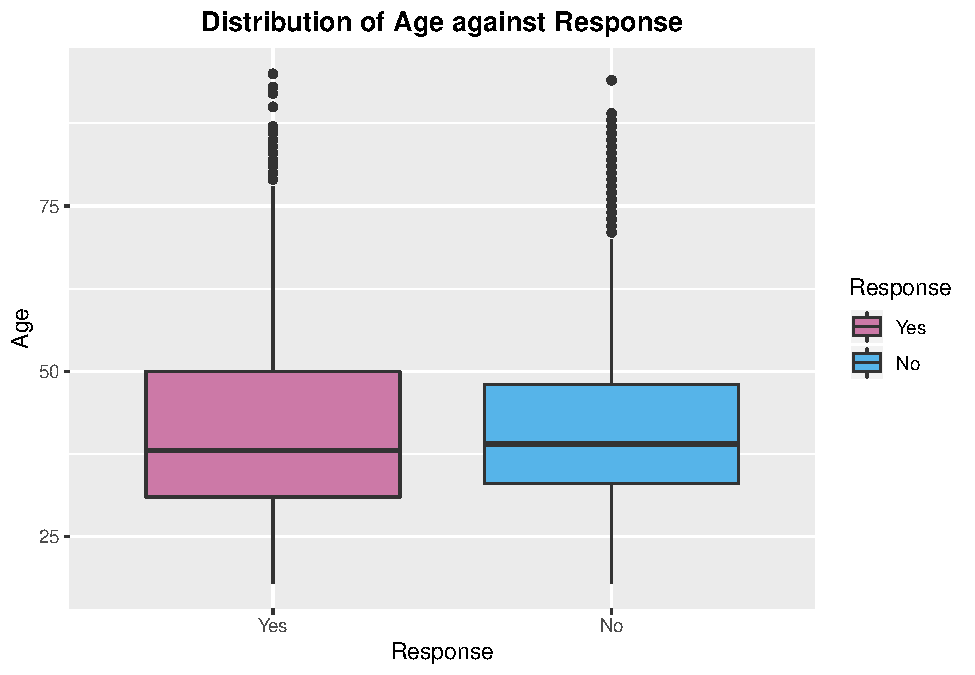
\includegraphics{CompiledTechnicalReport_files/figure-latex/unnamed-chunk-3-1} 

}

\caption{Age distribution of respondents against response in the second study}\label{fig:unnamed-chunk-3}
\end{figure}

To compare the results with the first study, we further obtained the
95\% confidence intervals for the age of people in two populations as
delineated by whether they are willing to purchase the product. We are
95\% confident that respondents who agree to purchase the product are
from 23 to 74 years old, and those who refuse to purchase the product
are from 25 to 60 years old. As provided in the first study, the mean
age of individuals who agree to purchase the product is 25.5, falling
fairly close to the lower bound of the 95\% confidence interval in the
second study, so it's likely that people who are willing to buy the
products from the two studies are not representing the same population.
However, the mean age of respondents who refused to buy the product is
37.5, which is close to the mean age of the counterpart in the second
study (39 years old). Overall, we believe that based on age, samples in
the two studies are unlikely from the same population.

Next, to determine whether the choice to purchase the product is
statistically associated with another numeric variable non-mortgage loan
balance in the second study, we generated a density plot to compare the
age distribution of respondents who are willing to purchase the product
against those who are not, as is shown in Figure 3. The graph indicates
that both distributions are right skewed, and they overlap to a great
proportion with the distribution of respondents who refuse to buy the
product being slightly less right skewed. It can be inferred that
respondents who refused to buy the product might have a lightly lower
balance on average, and as verified by Welch Two sample t-test, the true
means of two populations are significantly different.

\begin{figure}

{\centering 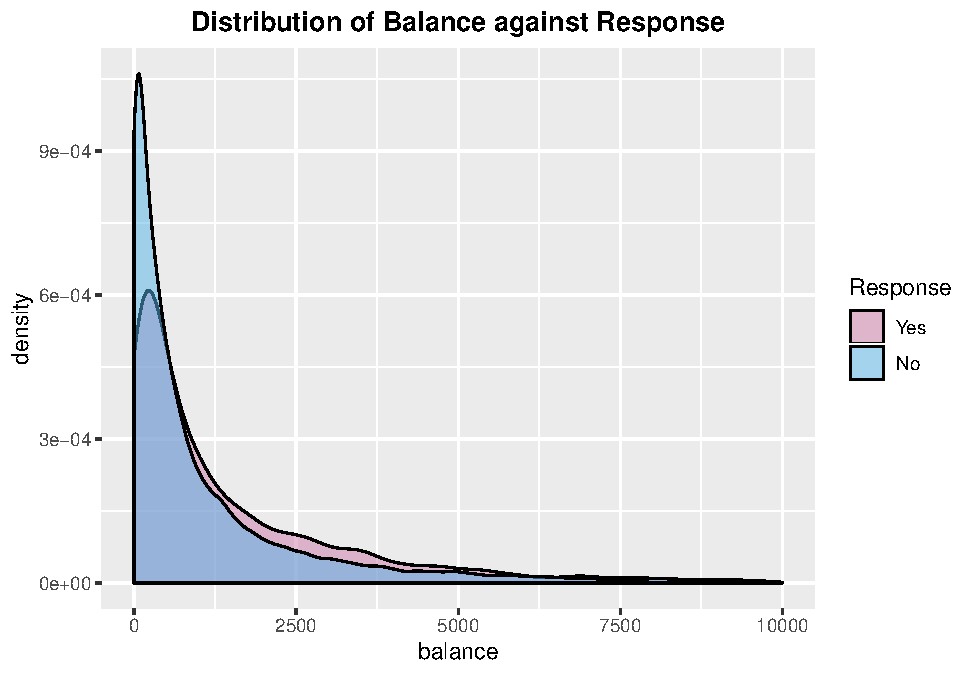
\includegraphics{CompiledTechnicalReport_files/figure-latex/unnamed-chunk-4-1} 

}

\caption{Distribution of non-mortgage loan balance against response in the second study}\label{fig:unnamed-chunk-4}
\end{figure}

We also obtained the 95\% confidence intervals for the non-mortgage loan
balance of people in two populations as delineated by whether they are
willing to purchase the product. We are 95\% confident that in the
second study, respondents who agree to purchase the product have
non-mortgage loan balance between -157.45 and 10185 USD, and those who
refuse to purchase the product have non-mortgage loan balance between
-393 and 8266 USD. Similar to the varible age, the average non-mortgage
loan balance of individuals who refuse to purchase the product (1250
USD) in the first study falls within the 95\% confidence interval of its
counterpart in the second study. However, the average non-mortgage loan
balance of individuals who agree to purchase the product is 23879 USD,
being way higher than the upper limit of its counterpart in the second
study, the sample in the first study is unlikely from the same
population of the second study.

Next, that, we continued to compare the categorical variable job in both
studies. Figure 4 shows the number of respondents of each type of job in
the second study as delineated by their responses to buy the product,
which is ranked by the order of counts in the refusal group from high to
low. Regardless of the reponse, it appears that most of the respondents
are blue-collar, technician or involved in management, but students and
households only take up a fairly small proportion of the sample.

\begin{figure}

{\centering 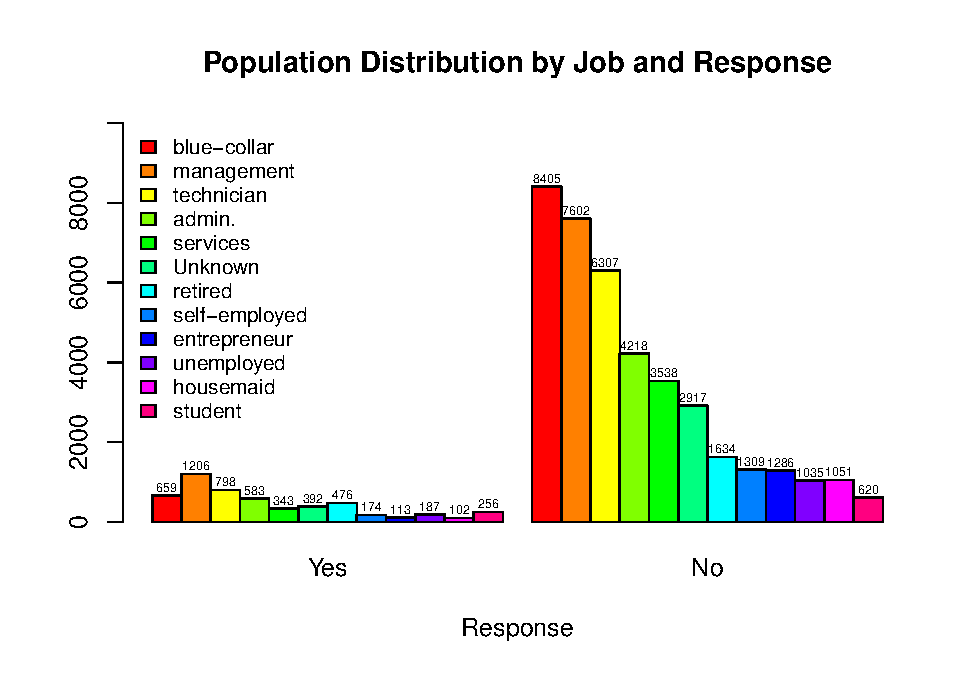
\includegraphics{CompiledTechnicalReport_files/figure-latex/unnamed-chunk-5-1} 

}

\caption{Population distribution of respondents by job and response in the second study}\label{fig:unnamed-chunk-5}
\end{figure}

\newpage

In order to allow for the comparison of job distributions in the two
studies, we collapsed blue-collar and technician into one category,
counted respondents who are entrepreneurs, administrators or involved in
management as white-collar and combined unemployed and unknown into one
category. Households and students are directly considered as single
levels of the job factor. With all the remaining job types omitted, we
generated barplots in Figure 5 to compare the distributions against
response. In stark contrast to what we observed for the second study, in
the first study, the most common job is student, whereas blue collars
are hardly seen. This clearly indicates that according to job type, the
two studies are not based on the same population.

\begin{figure}[h!]

{\centering \includegraphics{CompiledTechnicalReport_files/figure-latex/unnamed-chunk-7-1} 

}

\caption{Population distribution of respondents by job and response in both studies}\label{fig:unnamed-chunk-7}
\end{figure}

\newpage

We also compared the distribution of respondents with different
education backgrounds as delineated by their response to purchase the
product, as is shown in Figure 6. The tertiary education in the second
study can be regarded as the the same as the college and more level in
the first study, so the relevant bars were all highlighted in red. From
the figures, we can see that although there are similar numbers of
respondents who agree or refuse to buy the product in the first study,
in the second study there are more respondents with a non-favorable
response compared to a favorable response. The majority of the
respondents involved in the first study has education level of college
or higher, whereas in the second study, there's less respondents with
college education than respondents with secondary education. Based on
education levels, these two studies are not from the same population.

\begin{figure}[h!]

{\centering \includegraphics{CompiledTechnicalReport_files/figure-latex/unnamed-chunk-8-1} 

}

\caption{Population distribution of respondents by education and response in both studies}\label{fig:unnamed-chunk-8}
\end{figure}

Similarly, we also compared the distribution of respondents by marital
status against their response to purchase the product, as is shown in
Figure 7. In the first study, there're significantly lower numbers of
married respondents than unmarried respondents, whereas there are about
equal total numbers of married respondents as those unmarried in the
second study. Therefore, these two samples are unlikely from the same
population. Interestingly, if we focus on the distribution of married
respondents in both studies, married respondents are less likely to
purchase the product.

\begin{figure}

{\centering \includegraphics{CompiledTechnicalReport_files/figure-latex/unnamed-chunk-9-1} 

}

\caption{Population distribution of respondents by marital status and response in both studies}\label{fig:unnamed-chunk-9}
\end{figure}

\newpage

Furthermore, we compared the distribution of respondents with or without
mortgage against their response to purchase the product, as is shown in
Figure 8. Similar to what we observed in Figure 7, in the first study,
the majority of the respondents are without mortgage, whereas in the
second study there are about comparable number of respondents who have
mortgage or not. This could serve as edividence to show that the second
study was well designed to randomize the sample. In both studies, people
with mortgage are less likely to purchase the product as compared to
those with no mortgage. A possible explanation for this is that people
with mortgage could be more prudent with how they should spend money.
However, we see conflicting trends of response in the two studies among
the group with no mortgage, which could result from the difference in
sampling.

\begin{figure}

{\centering \includegraphics{CompiledTechnicalReport_files/figure-latex/unnamed-chunk-10-1} 

}

\caption{Population distribution of respondents by mortgage and response in both studies}\label{fig:unnamed-chunk-10}
\end{figure}

Figure 9 represents the distribution of respondents who use cell phones
as their primary phone against their response to purchase the product.
Less than half of the respondents use cell phone as their primary phone
in the first study, whereas more than half of the respondents use cell
phone as their primary phone in the second study. The second study may
be representing the true population, as nowadays people tend to use cell
phone more often than before. Interestingly, although respondents who
use cell phones as their primary phone tend to agree to buy the product
in the first study, this trend is reversed in the second study, with the
majority of the respondents refused to buy the product. This could
server as more evidence that these two samples are not from the same
population.

\begin{figure}

{\centering \includegraphics{CompiledTechnicalReport_files/figure-latex/unnamed-chunk-11-1} 

}

\caption{Population distribution of respondents by primary phone and response in both studies}\label{fig:unnamed-chunk-11}
\end{figure}

\newpage

It's possible that people in delinquency for more than 60 days also have
credit default, so we compared the delinquency variable in the first
study with the credit in default varible in the second study, as is
shown in Figure 10. The majority of the respondents in the second study
do not have credit in default. Comparatively, slighly more than half of
the respondents in the first study have less than 60 days of
delinquency. Interestingly, in the first study, respondents that have
less than 60 days of delinquency are less likely to buy the products. A
similar trend is observed in the second study, where the majority of
repondents with no credit in default refuse to buy the product.

\begin{figure}

{\centering \includegraphics{CompiledTechnicalReport_files/figure-latex/unnamed-chunk-12-1} 

}

\caption{Comparison of the population distribution by delinquency and response in the first study against the population distribution by credit in default and response in the second study}\label{fig:unnamed-chunk-12}
\end{figure}

Now that the variables common in both studies have been compared, we
continued to examine the pattern of distributions with variables only
described in the first study, including gender and race. Figure 11
displays the side-by-side distribution of respondents of different
gender or race against response. Males and white individuals are
overrepresented in this study, which could potentially lead to biased
response rates.

\begin{figure}

{\centering \includegraphics{CompiledTechnicalReport_files/figure-latex/unnamed-chunk-13-1} 

}

\caption{Population distribution of respondents by gender against response or by race against response in the first study}\label{fig:unnamed-chunk-13}
\end{figure}

In the second study, personal loan status is the only variable reflecing
demographic features that has yet to be investigated. Consistent with
what we observed for the credit in default variable, the majority of the
respondents are with no personal non-mortgage loans as shown in Figure
12. Interestingly, regardless of having personal loan or not, they both
tend to not buy the product, with similar probabilities.

\begin{figure}

{\centering \includegraphics{CompiledTechnicalReport_files/figure-latex/unnamed-chunk-14-1} 

}

\caption{Population distribution of respondents by personal loan and response in the second study}\label{fig:unnamed-chunk-14}
\end{figure}

\newpage

\hypertarget{likelihood-ratio-tests}{%
\subsubsection{Likelihood ratio tests}\label{likelihood-ratio-tests}}

Next, we conducted likelihood ratio tests to examine whether response to
purchase the product is dependent on each categorical variable
reflecting demographic features. Table 1 includes likelihood ratio test
statistics, degrees of freedom and p-values of the tests on the eight
variables (job, education, marital status, mortgage, primary phone,
delinquency, gender and race) for the first study. All of the p-values
are less than 0.05, indicating that there is significant evidence that
response to buy the product are associated with each of these eight
variables.

\begin{table}[h!]
    \centering
    \begin{tabular}{ |c | c | c | c | c |}
    \hline
        Variable & Levels & \(G^2\) & df & P-value \\ \hline
        Job & White Collar, Blue Collar, Student, House, Unemployed or Unknown & 321.67 & 4 & < 0.001 \\ \hline
        Education & College and more, Lower than college & 31.92 & 1 & < 0.001 \\ \hline
        Marital & Married, Not married & 71.97 & 1 & < 0.001 \\ \hline
        Mortgage & Mortgage, No Mortgage & 19.49 & 1 & <0.001 \\ \hline
        Primary Phone & Cellular, Other & 68.66 & 1 & <0.001 \\ \hline
        Delinquency & More than 60 days, 60 or less days & 113.33 & 1 & <0.001 \\ \hline
        Gender & Male, Female & 6.81 & 1 & 0.009 \\ \hline
        Race & White, Not White & 4.08 & 1 & 0.043 \\ \hline
    \end{tabular}
    \caption{Likelihood ratio tests of the dependence of response on the demographic variables in the first study}
\end{table}

Table 2 shows the likelihood ratio tests of whether response to purchase
the product is dependent on each of the demographic categorical variable
in the second study, including job, education, marital status, mortgage,
primary phone, credit in default and personal loan. The categories used
are based on the original levels of factors in the second study. Similar
to what we observed in Table 1, all of the p-values are less than 0.05,
suggesting that there is significant evidence that response to buy the
product are dependent on each of these seven variables.

\begin{table}[h!]
    \centering
    \begin{tabular}{ |c | c | c | c | c |}
    \hline
        Variable & Levels & \(G^2\) & df & P-value \\ \hline
        Job & \shortstack{Administer, Management, Entrepreneur, Blue-collar, \\  Technician, Student, Housemaid, Unemployed, \\ Unknown, Self-employeed, Services, Retired} & 698.03 & 11 & < 0.001 \\ \hline
        Education & Tertiary, Secondary, Primary,  Unknown & 226.34 & 3 & < 0.001 \\ \hline
        Marital & Married, Single, Divorced & 193.16 & 2 & < 0.001 \\ \hline
        Mortgage & Mortgage, No Mortgage & 868.71 & 1 & <0.001 \\ \hline
        Primary Phone & Cellular, Telephone, Unknown & 68.66 & 1 & <0.001 \\ \hline
        Credit in default & Credit in default, No credit in default & 24.33 & 1 & <0.001 \\ \hline
        Personal Loan & Personal Loan, No personal loan  & 232.1 & 1 & <0.001 \\ \hline
    \end{tabular}
    \caption{Likelihood ratio tests of the dependence of response on the demographic variables in the second study}
\end{table}

Since for response is statistically associated with each of the five
categorical variables common in both studies, we further conducted five
more likelihood ratio tests to examine whether the samples in the two
studies are from the same population. Assuming that they are two samples
from the same population, then the proportion of each level of the
interaction terms of response and any of the five categorical variables
should be the same for both studies. To allow for the comparisons, the
categories used are based on the original levels of factors in the first
study. The test statistics are shown in Table 3. As expected, the
p-values are all less than 0.05, which confirms that the components of
respondents in the first study are significantly different from that in
the well randomized second study.

\begin{table}[h!]
    \centering
    \begin{tabular}{ |c | c | c | c | c |}
    \hline
        Variable & Levels before interacted with Response & \(G^2\) & df & P-value \\ \hline
        Job & White Collar, Blue Collar, Student, House, Unemployed or unknown & 861348.2 & 9 & < 0.001 \\ \hline
        Education & College and more, Lower than College & 82340.45 & 3 & < 0.001 \\ \hline
        Marital & Married, Not married & 82723.05 & 3 & < 0.001 \\ \hline
        Mortgage & Mortgage, No Mortgage & 80419.45 & 3 & <0.001 \\ \hline
        Primary Phone & Cellular, Other & 69783.29 & 3 & <0.001 \\ \hline
    \end{tabular}
    \caption{Likeliihood ratio test of whether the samples in teh twoo studies are from the same population}
\end{table}

\hypertarget{exploratory-data-analysis-for-modeling-process}{%
\subsection{Exploratory Data Analysis for Modeling
Process}\label{exploratory-data-analysis-for-modeling-process}}

For the model analysis of this study, we were interested in creating a
logistic model to estimate the likelihood that a person would buy the
product based off of their demographic information. This is in effort to
create a generalized model that can be used to predict the success of
the Toast-USB.

First, we want to explore the relationship between the demographic
variables in the sample, and particularly explore how demographic
information affects willingness to purchase Toast-USB. In this case, we
can define willingness to purchase the Toast-USB as both the binary
(Y/N) favorable response and the price a person said they would be
willing to pay for the product. Figure 13 shows the relationship between
age and willingness to purchase. There is a moderate relationship
between age and price. The figure suggests that individuals on the older
end of the spectrum may actually have a more favorable response to the
product. This is somewhat contradictory to our expectation, given that
Millennial and Gen-Z's dual love for technology and gourmet toast served
as a compelling reason to enter this market space with the launch of the
Toast-USB. This paradoxical relationship could be due to the fact that
younger people are more likely to eat-out rather than at home, and
therefore are less likely to purchase kitchen appliances. Additionally,
young people establishing their first household may have access to less
capital to purchase appliances, resulting in a decreased willingness to
purchase among this demographic group. The figure also demostrated that
people had a favorable response to the product were also, on average,
willing to pay more for the product.

Next, we explored the relationship between logged-balance and
willingness to purchase. Balance representes the amount of non-morgatage
credit currently owed by an individual. If a person has a large
negative-value balance, it could negatively impact their willingness to
purchase the Toast-USB simply because they do not have access to
capital. The metric representing balance had both negative values and is
strongly right-skewed. We performed a linear shift by the largest
negative-value balance and a log-transformation to alleviate the skew of
the date. The equation below represents the mathematical formula used to
transform the balance variable, and the density plot for this variable
is included in the appendix:

\[Transformed_Balance = log(Balance + min(Balance))\]

Figure 14 represents the association between logged balance and
willingness to purchase Toast-USB. The figure does not demonstrate that
there is a significant association between balance and willingness to
purchase. Similarly to the relationship demonstrated for age, the figure
also suggests that people with a favorable respone were, on average,
willing to pay more for Toast-USB.

\begin{figure}
\centering
\includegraphics{CompiledTechnicalReport_files/figure-latex/unnamed-chunk-15-1.pdf}
\caption{Association between age and willingness to purchase Toast-USB}
\end{figure}

Based on the analysis of the continuous demogrpahic predictors, none of
the variables have a particularly strong association with willingness to
purchase, and there are no obvious instances of collinearity. However,
the plots of the continuous predictors do suggest that price is a
significant seperator. As demonstrated in previous exploratory analysis,
individuals who had a favorable response to the product were also
willing to pay more for it than people who did not have an initial
favorable response.

Figure 15 shows the association between categorical demographic
predictors and their willingness to purchase the Toast-USB. Variables
representing education, default, and loan have a moderate relationship
with willingness to purchase. Individuals with secondary and tertiary
education have a higher favorable response rate, which could be dually
attributable to access to more capital and cultural trends surrounding
gourmet toast that are popular within this group. Additionally, there is
a moderate association between willingness to purchase, loan, and
default. We believe that these associations could be related, as
individuals with secondary and tertiary education (specifically,
individuals attended college) are more likely to have a non-morgatage
loan due to the exorbanant cost of education in the United States. The
association of these three variables should be considered in the
structure of the logistic model.

\begin{figure}
\centering
\includegraphics{CompiledTechnicalReport_files/figure-latex/unnamed-chunk-18-1.pdf}
\caption{Association categorical demographic predictors and willingness
to purchase Toast-USB}
\end{figure}

The original dataset obtained by the DOE had 12 factors representing the
job classification for individuals in the sample. The job variable was
recoded to represent more broad categories more closely related to
profession-type. Factor levels in the recoded dataset for
profession-type include classifications of student, unknown employment,
administration, white-collar, and blue-collar. Figure 16 represents the
distribution of favorable response for each of the profession types.
There is no significant association between favorable response and
profession type in this sample.

\begin{figure}
\centering
\includegraphics{CompiledTechnicalReport_files/figure-latex/unnamed-chunk-19-1.pdf}
\caption{Distribution of Recoded Job}
\end{figure}

After exploratory analysis, we believe that default status, education,
personal loan status, and age are demographic variables of interest that
could be utilized in the logistic model. For the statistical analysis
portion, we aim to build a logistic model that uses relevant demographic
variables to predict a favorable response to the Toast-USB and indicate
if Toast-Co.~should move forward with the launch of the produce.

\hypertarget{generation-of-logistic-models-and-model-selection-by-cross-validation}{%
\subsubsection{Generation of Logistic Models and Model Selection by
Cross
Validation}\label{generation-of-logistic-models-and-model-selection-by-cross-validation}}

We identified that default status, education, personal loan status, and
age were potentially significant indicators of willingness to purchase
in the exploratory analysis. Our aim for the analysis was to 1) predict
the success of the Toast-USB and 2) indicate which demographic groups
should be targeted in the marketing campaign. To investigate these
endpoints, we generated a function that build a multivariate logistic
models representing every combination of the four aforementioned
variables. Interaction terms were not included, as none of these
variables demonstrated significant collinearity. We partitioned the data
into a test and a train set, both of which represented half of the
original dataset (non-overlapping) to be used for cross validation.
Using the train-set, we generated 15 potential logistic models
representing combinations of these four predictors. Next, we generated a
function to cross-validate the models using the test-set to select the
model with the maximal likelihood ratio.

\begin{verbatim}
## y ~default+education 
##                    5
\end{verbatim}

\begin{verbatim}
## 
## Call:
## glm(formula = bestFormula, family = binomial, data = training)
## 
## Deviance Residuals: 
##     Min       1Q   Median       3Q      Max  
## -0.6869  -0.5324  -0.4907  -0.4141   2.5376  
## 
## Coefficients:
##                     Estimate Std. Error z value Pr(>|z|)    
## (Intercept)        -2.074487   0.119146 -17.411  < 2e-16 ***
## educationprimary   -0.536865   0.101331  -5.298 1.17e-07 ***
## educationsecondary -0.185907   0.085009  -2.187  0.02875 *  
## educationtertiary   0.215881   0.086531   2.495  0.01260 *  
## loanUnkown          0.018640   0.197521   0.094  0.92482    
## loanyes            -0.717805   0.070499 -10.182  < 2e-16 ***
## age                 0.006008   0.002023   2.970  0.00297 ** 
## ---
## Signif. codes:  0 '***' 0.001 '**' 0.01 '*' 0.05 '.' 0.1 ' ' 1
## 
## (Dispersion parameter for binomial family taken to be 1)
## 
##     Null deviance: 16450  on 22604  degrees of freedom
## Residual deviance: 16177  on 22598  degrees of freedom
## AIC: 16191
## 
## Number of Fisher Scoring iterations: 5
\end{verbatim}

Of the 15 logistic models that were generated using the four key
demographic variables, we found that the multivariate logistic model
regressing age, personal loan status, and education on response to
Toast-USB had the maximum likelihood ratio. The model summary also
indicated that all of these predictors have a significant effect on the
favorable response rate. Thus, we believe that education, loan status,
and age will be demographic variables of interest to Toast-Co for
strategizing their marketing campaign. Next,we used our selected
logistic model to simulate a response rate using the testing set.

\begin{verbatim}
## [1] 0.1191772
\end{verbatim}

The favorable response rate for for the product was 12.14\%, which is
approximately half of the necessary response rate that
Toast-Co.~indicated would be necessary for the launch of the product.
Based on this analysis, we do not recommend that Toast Co.~move forward
with this version to Toast-USB.

\hypertarget{application-of-model-to-determine-msrp}{%
\subsection{Application of Model to Determine
MSRP}\label{application-of-model-to-determine-msrp}}

From our previous section, we discovered that the logistic model
containing personal loan status, education, and age as predictor
variables performs the best predictions according to maximum likelihood
ratio. Although the favorable response is below the break even rate, we
still determined which MSRP value would be able to maximize revenue. To
generate a range of reasonable prices, we selected the minimum and
maximum value of price answered in the survey. The lowest value
responded value was 0, so we started our search at 1 USD. The maximum
responded price was 168 USD. Thus, the range for reasonable prices was
determined to be {[}1-168 USD{]}. To find the maximum price we performed
the following simulation

For each potential MSRP Value, repeat the below following process 5
times and take the average: For each observation in our training set: 1.
Generate a probability they would purchase the product using the
logistic model 2. Compare that generated probability with a randomly
generated number, if the random number is lower than the probability
then the customer will consider purchasing the item. If not then we skip
to next observation. 3. We compare the MSRP to observed price the
customer said they were willing to pay. If the MSRP is less than than
the price then in our simulation the customer ``purchases'' the product
and that sale is added to the total revenue and we continue to the next
observation. We key the total revenue to be associated with the MSRP
value and selected the MSRP value with the highest revenue.

\includegraphics{CompiledTechnicalReport_files/figure-latex/unnamed-chunk-22-1.pdf}

From the results of our simulation we can see that the estimated maximum
MSRP Value would 46 USD. The simulation was ran on a test set containing
20,000 observations. From this we could estimate that for every 20,000
people that interact with our product we could estimate a revenue of
approximately 60,000 USD.

\hypertarget{discussion-and-conclusion}{%
\subsection{Discussion and Conclusion}\label{discussion-and-conclusion}}

Toast is a staple in the American diet. It is an extremely popular
breakfast food, and in recent years has gained even more popularity, as
artisanal toast is at the center of Millennial and Gen-Z dietary trends.
Our client, ToastCo., has proposed the launch of the Toast-USB, which
would allow amateursand toast connoisseurs alike to create
culinary-grade toast straight from theircomputer. Our aim was was to
assist Toast-Co.~to make data-driven, insightful decisions regarding the
launch and campaign strategy for this product. In particular, we has
three specific aims for the analysis.

\begin{enumerate}
\def\labelenumi{\arabic{enumi}.}
\item
  Compare the demographic and campaign-specifc features from the two
  samples quantitatively and qualitatively.
\item
  Make a binary (Y/N) recommendation regarding launch of the product
  based on a selection of significant demographic predictors and
  logistic modeling.
\item
  Determing an MSRP that will maximize revenue for the product.
\end{enumerate}

In the intitial analysis, we compared the demographic features of the
first and second study. For the two numeric variables common in both
studies, we obtained distribution plots and 95\% confidence intervals of
age and non-mortgage loan balance in the second study, and then compared
them to the mean of age and non-mortgage loan balance in the second
study. The results suggests that based on age and non-mortgage loan
balance, samples in the two studies are unlikely from the same
population.

We further compared the categorical variables common in both studies,
including job, education, marital status, mortgage and primary phone.
Students are overrepresented whereas blue collar workers are
underrepresented in the first study, which is opposite to what we've
observed in the second study. Individuals with education levels of
college and more are overrepresented, whereas married individuals or
individuals with mortgage are underrepresented in the first study. Also,
respondents using cell phone as the primary phone are slightly
underrepresented in the first study.

There are two categorical variables only present in the first study,
including gender and race. White males appear to overrepresent the
respondents. For the the second study, people with no personal loan take
up a great proportion.

After that, likelihood ratio tests have verified that there is
significant evidence that response to buy the product are associated
with all the demographic variables in both studies, and that the
components of respondents in the first study are significantly different
from that in the well randomized second study.

We performed further exploratory analysis on the data from the second
study to gain insights on which demographic variables would have a
meaningful effect on the favorable response rate. We found that age,
personal loan status, default status and education were key demographic
features of interest for the marketing campaign. We built 15 logistic
models using combinations of these variables, and found that the
logistic model including age, personal loan status, and education had
the maximum likelihood ratio. Based on this result and the exploratory
analysis, the Toast-USB has the highest favorble response rate among
older individuals with higher levels of education and access to capital
(no defaulted debt).

We performed a simulation on the test set to determing the estimated
favorable response rate. The estimated response rate for this sample was
12.14\%, which was under the 24.13\% benchmark that is required to
break-even. Based on this result, we do not recommend that Toast
Co.~proceed with the launch of the Toast-USB. This result was somewhat
contradictory to the results of the first study, which had extremely
promising preliminary findings and a 50.36\% favorable response rate.
Our investigation into the quantitative and qualitative differences
betweent the first and second study suggested that the first study was
not representative of the true population, and overrepresentation of
certain groups led to bias in the favorable response rate of that study.

Despite the recommendation to not proceed with this campaign, we believe
that the investigation into the MSRP for the product to maximize revenue
could be useful for the Toast Co., should they decide to launch a
similar product in the future. We performed a simulation using the
probability that the individual would purchase the product calcualted
from the logistic model and the price that the individual cited that
they were willing to pay. Using this process, we determined that the
optimal price for this product is 46 USD, which would generate an
estimated revenue of 60,000 USD.

Although we do not recommend launching the Toast-USB, there are some key
insights that we found in this investigation that could potentially be
very useful to Toast Co.~in reevaluating their business strategy. Since
we believe that older, highly-educated indivuduals are most likely to
have a favorable response to the product, Toast Co.~could re-imagine the
Toast-USB to be more tailored to this group of people. This could
include adding more functional features, updating the aesthetic design,
or improving the software systems to the product.

\hypertarget{appendix}{%
\subsection{Appendix:}\label{appendix}}

\begin{table}[h!]
    \centering
    \begin{tabular}{| m{3.2cm} | m{2cm} | m{50mm}|}
    \hline
    \rowcolor{lightgray}
    Variable & Variable Type & Notes \\
    \hline
    Age & Numeric & Age of respondent in years.\\
    \hline
    Job & Categorical & Classification of jobs into 12 different categories.\\
    \hline
    Marital & Categorical & Indicates if respondent is Single, Married, or Separated.\\
    \hline
    Education & Ordinal & Respondents highest level of education. Ordered: Primary, Secondary, Tertiary.\\
    \hline
    Default &Binary& Indicator that respondent has defaulted on Credit.\\
    \hline
    Balance & Numeric & Amount of Non-mortgage credit currently borrowed.\\
    \hline
    Housing & Binary & Indicator that respondent has a mortgage.\\
    \hline
    Loan & Binary & Indicator that respondent has Non-mortgage loan.\\
    \hline
    Contact & Categorical & If respondent was contacted through Cellular Phone or Home Phone.\\
    \hline
    Duration & Numeric & How long previous contact with respondent was. (in Seconds)\\
    \hline
    Number of Current Contacts & Numeric & Number of times respondent was contacted during this campaign.\\
    \hline
    Previous Contact & Numeric & Number of days between contact in previous campaign and current campaign.\\
    \hline
    Number of Previous Contacts & Numeric & Number of times respondent was contacted in previous campaign.\\
    \hline
    Previous Outcomes & Categorical & Outcome of contact with respondent.\\
    \hline
    Will Purchase & Binary & If respondent would purchase the product.\\
    \hline
    Price & Numeric & Regardless if respondent would purchase the product, what price they think would be appropriate. (in USD)\\
    \hline
    In Previous Study & Binary & Indicator if respondents participated in previous campaign. \\
    \hline
    \end{tabular}
    \caption{Data Dictionary}
    \label{tab:my_label}
\end{table}

\begin{figure}
\centering
\includegraphics{CompiledTechnicalReport_files/figure-latex/unnamed-chunk-23-1.pdf}
\caption{Density distribution of transformed balance}
\end{figure}

\end{document}
